\documentclass[letterpaper,openany,oneside,twocolumn]{book}

\newcommand{\PATH}{../../}

\usepackage{fontspec}
\usepackage[justified]{\PATH dndtemplate/dnd}
\usepackage{ifthen}
\usepackage{pstricks}

\usepackage{intcalc}

\usepackage[UKenglish]{babel}
\usepackage{\PATH dndtemplate}

\setlength\oddsidemargin{\dimexpr(\paperwidth-\textwidth)/2 - 1in\relax}
\setlength\evensidemargin{\oddsidemargin}

% Headline
\CharacterName{Laucian Ilphelkiir}

\Class{Ranger}
\Level{12}
\Background{Folk Hero}
\PlayerName{M4RZ}
\Race{Wood Elf}
\Alignment{Chaotic Good}
\XP{}

% Ability scores
\StrengthScore{16}
\DexterityScore{20}
\ConstitutionScore{14}
\IntelligenceScore{16}
\WisdomScore{14}
\CharismaScore{14}

% Proficiencies (Proficient = 'P', Expertise = 'E', otherwise = '')
\StrengthProficiency{P}
\DexterityProficiency{P}
\ConstitutionProficiency{}
\IntelligenceProficiency{}
\WisdomProficiency{}
\CharismaProficiency{}

\AcrobaticsProficiency{}
\AnimalHandlingProficiency{P}
\ArcanaProficiency{}
\AthleticsProficiency{P}
\DeceptionProficiency{}
\HistoryProficiency{}
\InsightProficiency{}
\IntimidationProficiency{}
\InvestigationProficiency{}
\MedicineProficiency{}
\NatureProficiency{P}
\PerceptionProficiency{P}
\PerformanceProficiency{}
\PersuasionProficiency{}
\ReligionProficiency{}
\SleightOfHandProficiency{}
\StealthProficiency{P}
\SurvivalProficiency{P}

\Inspiration{}
\Proficiency{+4}

\ArmorClass{17}
\InitiativeModifier{0}
\Speed{35ft}
\MaxHitPointsRolled{83}
\CurrentHitPoints{}
\TemporaryHitPoints{}
\HitDice{d10}
\HitDiceSpent{0}

\CP{}
\SP{}
\EP{}
\GP{3633}
\PP{}


\AddWeapon{2 Shortswords}{0}{1d6 p}
\AddWeapon{Anletta's Bow}{+1}{1d8 p}

\AttacksAdditional{
	\textbf{Anletta's Bow:}\\+1 Damage against Undead\\
	\textbf{60 Arrows} (1 with Oil)\\
	\textbf{Boomerang Arrow}\\
	\textbf{50 Fire Arrows}\\
	\textbf{5 Ice Arrows}\\
	\textbf{Armor:}\\Chain Shirt +2, Leather Armor\\
}

\OtherProficienciesLanguages{
	\textbf{Languages:}\\Common, Elvish, Sylvan, Draconic\\
	\textbf{Armor:}\\Light, Medium Armor, Shields\\
	\textbf{Weapons:}\\Shortsword, Longsword, Shortbow, Longbow, Simple, Martial Weapons\\
	\textbf{Tools:}\\Woodcarver's Tools
}

\Equipment{
	\small{Woodcarver's Tools,
	a Shovel,
	an Iron Pot,
	Set of Common Clothes,
	a Backpack,
	a Bedrool,
	a Mess Kit,
	a Tinderbox,
	10 Torches,
	12 Days of Rations,
	a Waterskin,
	50 ft Hempen Rope,
	Firewine,
	a Tranquilizer Vial,
	Wedge Stone (Arrows +1/+2 Damage),
	a Potion of Greater Healing,
	a Potion of Supreme Healing,
	Ruby (500 gold) \\
	\textbf{
	Quiver of Ehlonna,
	Manual of Gainful Exercise (used),
	Ioun Stone: Insight,
	Wand of Secrets}
	}
}

\PersonalityTraits{
	I'm confident in my own abilities and do what I can to instill confidence in others.
}

\Ideals{
	Nature is worth protecting and all animals are precious \\
	\textbf{Destiny.} Nothing and no one can steer me away from my higher calling.
}

\Bonds{
	I want to uncover what happened to my old tribe \\
	I worked the land, I love the land, and I will protect the land.
}

\Flaws{
	Afraid of Fire and very revengeful, easily raged.
}

\FeaturesTraits{
\textbf{Elf Traits}
\begin{itemize}
	\item Darkvision
	\item Fey Ancestry
	\item Trance
	\item Elf Weapon Training
	\item Mask of the Wild
\end{itemize}
\textbf{Favored Enemy}
\begin{itemize}
	\item Elementals, Dragon
\end{itemize}
\textbf{Favorable Terrain}
\begin{itemize}
	\item Forest, Swamp, Arctic, Mountain
\end{itemize}
\textbf{Fighting Style}
\begin{itemize}
	\item Archer
\end{itemize}
\textbf{Ranger Archetypes}
\begin{itemize}
	\item Horde Breaker
	\item Escape the Horde
	\item Volley
\end{itemize}
\textbf{Feats}
\begin{itemize}
	\item Sharpshooter
	\item Wood Elf Magic
\end{itemize}
}

% Appearance

\Age{240}
\Height{6'2"}
\Weight{110lbs}
\Eyes{Silver}
\Skin{Greenish}
\Hair{Brown}

% background

\CharacterAppearance{
	\begin{center}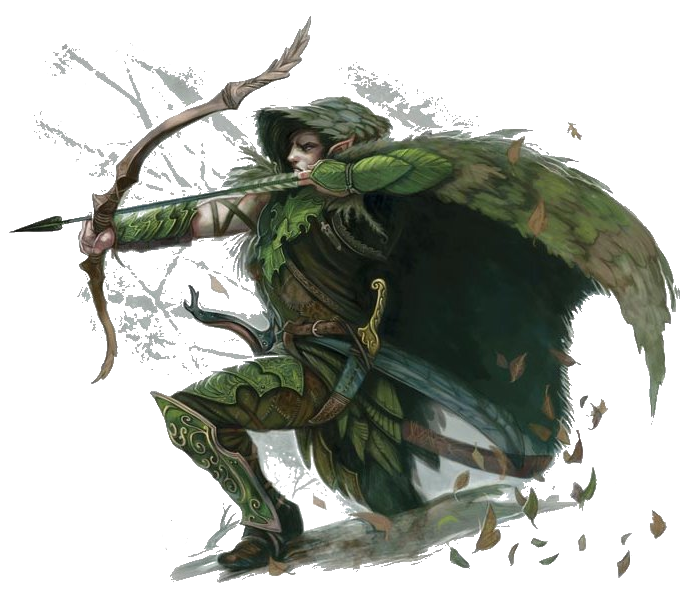
\includegraphics[width=160pt]{images/Laucian_Ilphelkiir.png}\end{center}
	\noindent Laucian’s silver eyes glisten like his bow. He has short, brown hair. He has long, pointed ears that prick up when Laucian is on the hunt or guard.
}
\AdditionalFeaturesAndTraits{
Laucian is very capable of climbing trees and scaling natural barricades. Also, he is very gifted with a bow and arrow and very talented in hunting game and gathering food while in nature. Furthermore, he learned to camouflage himself and to be very stealthy while stalking his prey and enemies.
}
\Characterbackground{
Laucian was born an elf of the wood - a very reclusive race that dwells in the forests of "Eastern Wallaby Grove". His parents were aristocrats of the tribe whereas his grandfather was the main hunter of the community. Because of his grandfather's teachings, Laucian quickly became an expert marksman with the bow and also in laying traps for wild animals. As Laucian was very capable at a young age he was very respected since he provided the clan with venison and other sorts of foods that were gathered during the seasonal hunt. \\
The most striking event was when Laucian was just 40 years old. On that particular day, the city of "New Forestia" was attacked by a huge dragon that burned down everything that stood in its way. Laucian was the only survivor on that faithful day and he became obsessed with the search for that dragon. Also, he became afraid of the nature of fire as he observed the obstruction it was capable of.
}
\Treasure{
A small pouch with a single silver piece with the old stamping of "New Forestia" and a talisman with the symbol of the tribe.
}
\AlliesAndOrganizations{
The clan of "New Forestia" was once a very flourishing and wealthy tribe. Although, the main population of the tribe lived very reclusive trade with surrounding tribes prospered and the yield of hunts was a very popular commodity in the nearby villages and cities. \\
On a faithful day, nearly 200 years ago the tribe and the whole forest of "Eastern Wallaby Grove" were burned down by the Dragon "Braga, the Red". Laucian Ilphelkiir, a son of the noblemen of the clan was the only survivor and tries to find allies and friends of "New Forestia" to spread the knowledge of what happened and that the history of this once prospering tribe is never forgotten.
}
\OrganizationName{New Forestia (Elf Tribe)}
\OrganizationSymbol{images/Tree_of_Forestia.jpg}

% Magic

\SpellcastingClass{Ranger}
\SpellcastingAbility{WIS} % STR, DEX, CON, INT, WIS, CHA
\SpellSaveDCModifier{0} % any modifier that isn't contained in "8 + Ability Modifier + Proficiency Bonus"

\CantripSlotA{Control Flames (S)}

\FirstLevelSpellSlotsTotal{4}
\FirstLevelSpellSlotA{Ensnaring Strike (V)}
\FirstLevelSpellSlotB{Hail of Thorns (V)}
\FirstLevelSpellSlotC{Longstrider (V, S, M) (once a day)}

\SecondLevelSpellSlotsTotal{3}
\SecondLevelSpellSlotA{Find Traps (V, S)}
\SecondLevelSpellSlotB{Spike Growth (V, S, M)}
\SecondLevelSpellSlotC{Cordon of Arrows (V, S, M)}
\SecondLevelSpellSlotD{Pass Without Trace (V, S, M) (once a day)}

\ThirdLevelSpellSlotsTotal{3}
\ThirdLevelSpellSlotA{Lightning Arrow (V, S)}
\ThirdLevelSpellSlotB{Conjure Barrage (V, S, M)}
\ThirdLevelSpellSlotC{Protection from Energy (V, S)}

\begin{document}

\newgeometry{left=0cm,right=0cm,top=0cm,bottom=0cm}
\onecolumn


% CHARACTER PAGE
\rendercharactersheet

% BACKSTORY PAGE
\renderbackgroundsheet

% SPELLCASTING PAGE
\renderspellsheet



\restoregeometry
\twocolumn

\chapter*{Features, Magic Items and Spells}

\section*{Ranger}
\subsection*{Favored Enemy}
You have significant experience studying, tracking, hunting, and even talking to a certain type of enemy.

Choose a type of favored enemy: aberrations, beasts, celestials, constructs, dragons, elementals, fey, fiends, giants, monstrosities, oozes, plants, or undead. Alternatively, you can select two races of humanoid (such as gnolls and orcs) as favored enemies.

You have advantage on Wisdom (Survival) checks to track your favored enemies, as well as on Intelligence checks to recall information about them.

When you gain this feature, you also learn one language of your choice that is spoken by your favored enemies, if they speak one at all.

You choose one additional favored enemy, as well as an associated language, at 6th and 14th level. As you gain levels, your choices should reflect the types of monsters you have encountered on your adventures.

\subsection*{Natural Explorer}
You are particularly familiar with one type of natural environment and are adept at traveling and surviving in such regions. Choose one type of favored terrain: arctic, coast, desert, forest, grassland, mountain, swamp, or the Underdark. When you make an Intelligence or Wisdom check related to your favored terrain, your proficiency bonus is doubled if you are using a skill that you're proficient in.

While traveling for an hour or more in your favored terrain, you gain the following benefits:
\begin{itemize}
	\item Difficult terrain doesn't slow your group's travel.
	\item Your group can't become lost except by magical means.
	\item Even when you are engaged in another activity while traveling (such as foraging, navigating, or tracking), you remain alert to danger.
	\item If you are traveling alone, you can move stealthily at a normal pace.
	\item When you forage, you find twice as much food as you normally would.
	\item While tracking other creatures, you also learn their exact number, their sizes, and how long ago they passed through the area.
\end{itemize}
You choose additional favored terrain types at 6th and 10th level.

\subsection*{Fighting Style}
You adopt a particular style of fighting as your specialty. Choose one of the following options.

You can't take a Fighting Style option more than once, even if you later get to choose again.

\subsubsection*{Archery}
You gain a +2 bonus to attack rolls you make with ranged weapons.

\subsection*{Ranger Archetypes}
\subsubsection*{Hunter}
Emulating the Hunter archetype means accepting your place as a bulwark between civilization and the terrors of the wilderness. As you walk the Hunter's path, you learn specialized techniques for fighting the threats you face, from rampaging ogres and hordes of orcs to towering giants and terrifying dragons.

\paragraph*{Hunter's Prey}
\subparagraph*{Horde Breaker}
Once on each of your turns when you make a weapon attack, you can make another attack with the same weapon against a different creature that is within 5 feet of the original target and within range of your weapon.
\paragraph*{Defensive Tactics}
\subparagraph*{Escape the Horde}
Opportunity attacks against you are made with disadvantage.
\paragraph*{Multiattack}
\subparagraph*{Volley}
You can use your action to make a ranged attack against any number of creatures within 10 feet of a point you can see within your weapon's range. You must have ammunition for each target, as normal, and you make a separate attack roll for each target.

\subsection*{Primeval Awareness}
You can use your Action and expend one Ranger spell slot to focus your awareness on the region around you. For 1 minute per level of the spell slot you expend, you can sense whether the following types of Creatures are present within 1 mile of you (or within up to 6 miles if you are in your Favored terrain): Aberrations, Celestials, Dragons, Elementals, Fey, Fiends, and Undead. This feature doesn't reveal the creatures' Location or number.

\subsection*{Extra Attack}
You can Attack twice, instead of once, whenever you take the Attack Action on Your Turn.

\subsection*{Land's Stride}
Moving through nonmagical Difficult Terrain costs you no extra Movement. You can also pass through nonmagical Plants without being slowed by them and without Taking Damage from them if they have thorns, spines, or a similar hazard.

In addition, you have advantage on Saving Throws against Plants that are magically created or manipulated to impede Movement, such those created by the Entangle spell.

\subsection*{Hide in Plain Sight}
You can spend 1 minute creating camouflage for yourself. You must have access to fresh mud, dirt, Plants, soot, and other naturally occurring materials with which to create your camouflage.

Once you are camouflaged in this way, you can try to hide by pressing yourself up against a solid surface, such as a tree or wall, that is at least as tall and wide as you are. You gain a +10 bonus to Dexterity (Stealth) checks as long as you remain there without moving or taking ACTIONS. Once you move or take an Action or a Reaction, you must camouflage yourself again to gain this benefit.

\section*{Wood Elf Traits}
\subsection*{Darkvision}
Accustomed to twilit forests and the night sky, you have superior vision in dark and dim conditions. You can see in dim light within 60 feet of you as if it were bright light, and in darkness as if it were dim light. You can't discern color in darkness, only shades of gray.

\subsection*{Fey Ancestry}
You have advantage on saving throws against being charmed, and magic can't put you to sleep.

\subsection*{Trance}
Elves don't need to sleep. Instead, they meditate deeply, remaining semiconscious, for 4 hours a day. (The Common word for such meditation is “trance.”) While meditating, you can dream after a fashion; such dreams are actually mental exercises that have become reflexive through years of practice. After resting in this way, you gain the same benefit that a human does from 8 hours of sleep.

\subsection*{Elf Weapon Training}
You have proficiency with the longsword, shortsword, shortbow, and longbow.

\subsection*{Mask of the Wild}
You can attempt to hide even when you are only lightly obscured by foliage, heavy rain, falling snow, mist, and other natural phenomena.

\section*{Background}
\subsection*{Folk Hero}
You come from a humble social rank, but you are destined for so much more. Already the people of your home village regard you as their champion, and your destiny calls you to stand against the tyrants and monsters that threaten the common folk everywhere.

\subparagraph*{Skill Proficiencies} Animal Handling, Survival
\subparagraph*{Tool Proficiencies} One type of artisan's tools, vehicles (land)
\subparagraph*{Equipment} A set of artisan's tools (one of your choice), a shovel, an iron pot, a set of common clothes, and a pouch containing 10 gp

\section*{Feats}
\subsection*{Sharpshooter}
You have mastered ranged weapons and can make shots that others find impossible. You gain the following benefits:
\begin{itemize}
  \item Attacking at long range doesn't impose disadvantage on your ranged weapon attack rolls.
  \item Your ranged weapon attacks ignore half and three-quarters cover.
  \item Before you make an attack with a ranged weapon that you are proficient with, you can choose to take a -5 penalty to the attack roll. If that attack hits, you add +10 to the attack's damage.
\end{itemize}

\subsection*{Wood Elf Magic}
You learn the magic of the primeval woods, which are revered and protected by your people. You learn one Druid cantrip of your choice. You also learn the Longstrider and Pass Without Trace spells, each of which you can cast once without expending a spell slot. You regain the ability to cast these two spells in this way when you finish a long rest. Wisdom is your spellcasting ability for all three spells.

\section*{Magical Items}
\subsection*{Quiver of Ehlonna}
\textit{wondrous item, uncommon}

Each of the quiver's three compartments connects to an extradimensional space that allows the quiver to hold numerous items while never weighing more than 2 pounds. The shortest compartment can hold up to sixty arrows, bolts, or similar objects. The midsize compartment holds up to eighteen javelins or similar objects. The longest compartment holds up to six long objects, such as bows, quarterstaffs, or spears.

You can draw any item the quiver contains as if doing so from a regular quiver or scabbard.

\subsection*{Manual of Gainful Exercise (used)}
\textit{wondrous item, very rare}

This book describes fitness exercises, and its words are charged with magic. If you spend 48 hours over a period of 6 days or fewer studying the book's Contents and practicing its guidelines, your Strength score increases by 2, as does your maximum for that score. The manual then loses its magic, but regains it in a century.

\subsection*{Ioun Stone: Insight}
\textit{wondrous item, very rare (requires attunement)}
The Insight Ioun Stone is an incandescent blue sphere. You can use an action to toss this stone into the air, it orbits your head at a distance of 1d3 feet. While this stone orbits, your Wisdom score increases by 2, to a maximum of 20. Another creature can use an action to grasp or snare the stone to separate it from you, either by making a successful attack roll against AC 24 or a successful DC 24 Dexterity (Acrobatics) check. You can use an action to seize and stow the stone, ending its effect.

A stone has AC 24, 10 hit points, and resistance to all damage. It is considered to be an object that is being worn while it orbits your head.

\subsection*{Wand of Secrets}
\textit{wondrous item, uncommon}
The wand has 3 Charges. While holding it. you can use an Action to expend 1 of its Charges, and if a Secret door or trap is within 30 feet of you, the wand pulses and points at the one nearest to you. The wand regains 1d3 expended Charges daily at dawn.

\section*{Spells}

\subsection*{Bonus Spells}

\DndSpellHeader
  {Longstrider}
  {1st-Level Transmutation}
  {1 Action}
  {Touch}
  {V S M (A pinch of dirt)}
  {1 hour}

You touch a creature. The target's speed increases by 10 feet until the spell ends.

\subparagraph*{At Higher Levels} When you cast this spell using a spell slot of 2nd level or higher, you can target one additional creature for each slot level above 1st.

\DndSpellHeader
  {Pass Without Trace}
  {2nd-Level Abjuration}
  {1 Action}
  {Self}
  {V S M (Ashes from a burned leaf of mistletoe and a sprig of spruce)}
  {Concentration, up to 1 hour}

A veil of shadows and silence radiates from you, masking you and your companions from detection. For the duration, each creature you choose within 30 feet of you (including you) has a +10 bonus to Dexterity (Stealth) checks and can't be tracked except by magical means. A creature that receives this bonus leaves behind no tracks or other traces of its passage.

\subsection*{Cantrips}

\DndSpellHeader
  {Control Flames (Lessened)}
  {Druidic Cantrip}
  {1 Action}
  {60 feet (3 ft cube)}
  {S}
  {Instantaneous}

You choose nonmagical flame that you can see within range and that fits within a 3-foot cube. You affect it in one of the following ways:
\begin{itemize}
	\item You instantaneously expand the flame 3 feet in one direction, provided that wood or other fuel is present in the new location.
	\item You instantaneously extinguish the flames within the cube.
	\item You double or halve the area of bright light and dim light cast by the flame, change its color, or both. The change lasts for 1 hour.
	\item You cause simple shapes—such as the vague form of a creature, an inanimate object, or a location—to appear within the flames and animate as you like. The shapes last for 1 hour.
\end{itemize}
If you cast this spell multiple times, you can have up to three of its non-instantaneous effects active at a time, and you can dismiss such an effect as an action.


\subsection*{Level 1}

\DndSpellHeader
  {Ensnaring Strike}
  {1st-Level Conjuration}
  {1 Bonus Action}
  {Self}
  {V}
  {Concentration, up to 1 minute}

The next time you hit a creature with a weapon attack before this spell ends, a writhing mass of thorny vines appears at the point of impact, and the target must succeed on a Strength saving throw or be restrained by the magical vines until the spell ends. A Large or larger creature has advantage on this saving throw. If the target succeeds on the save, the vines shrivel away.

While restrained by this spell, the target takes 1d6 piercing damage at the start of each of its turns. A creature restrained by the vines or one that can touch the creature can use its action to make a Strength check against your spell save DC. On a success, the target is freed.

\subparagraph*{At Higher Levels} If you cast this spell using a spell slot of 2nd level or higher, the damage increases by 1d6 for each slot level above 1st.

\DndSpellHeader
  {Hail of Thorns}
  {1st-Level Conjuration}
  {1 Bonus Action}
  {Self}
  {V}
  {Concentration, up to 1 minute}

The next time you hit a creature with a ranged weapon attack before the spell ends, this spell creates a rain of thorns that sprouts from your ranged weapon or ammunition. In addition to the normal effect of the attack, the target of the attack and each creature within 5 feet of it must make a Dexterity saving throw. A creature takes 1d10 piercing damage on a failed save, or half as much damage on a successful one.

\subparagraph{At Higher Levels} If you cast this spell using a spell slot of 2nd level or higher, the damage increases by 1d10 for each slot level above 1st (to a maximum of 6d10).

\subsection*{Level 2}

\DndSpellHeader
  {Find Traps}
  {2nd-Level Divination}
  {1 Action}
  {120 feet}
  {V S}
  {Instantaneous}

You sense the presence of any trap within range that is within line of sight. A trap, for the purpose of this spell, includes anything that would inflict a sudden or unexpected effect you consider harmful or undesirable, which was specifically intended as such by its creator. Thus, the spell would sense an area affected by the alarm spell, a glyph of warding, or a mechanical pit trap, but it would not reveal a natural weakness in the floor, an unstable ceiling, or a hidden sinkhole.

This spell merely reveals that a trap is present. You don't learn the location of each trap, but you do learn the general nature of the danger posed by a trap you sense.

\DndSpellHeader
  {Spike Growth}
  {2nd-Level Transmutation}
  {1 Action}
  {150 feet}
  {V, S, M (seven sharp thorns or seven small twigs, each sharpened to a point)}
  {Concentration, up to 10 minutes}

The ground in a 20-foot radius centered on a point within range twists and sprouts hard spikes and thorns. The area becomes difficult terrain for the duration. When a creature moves into or within the area, it takes 2d4 piercing damage for every 5 feet it travels.

The transformation of the ground is camouflaged to look natural. Any creature that can't see the area at the time the spell is cast must make a Wisdom (Perception) check against your spell save DC to recognize the terrain as hazardous before entering it.

\DndSpellHeader
  {Cordon of Arrows}
  {2nd-Level Transmutation}
  {1 Action}
  {5 feet}
  {V, S, M (four or more arrows or bolts)}
  {8 hours}

You plant four pieces of nonmagical ammunition – arrows or crossbow bolts – in the ground within range and lay magic upon them to protect an area. Until the spell ends, whenever a creature other than you comes within 30 feet of the ammunition for the first time on a turn or ends its turn there, one piece of ammunition flies up to strike it. The creature must succeed on a Dexterity saving throw or take 1d6 piercing damage. The piece of ammunition is then destroyed. The spell ends when no ammunition remains.

When you cast this spell, you can designate any creatures you choose, and the spell ignores them.

\subparagraph{At Higher Levels} When you cast this spell using a spell slot of 3rd level or higher, the amount of ammunition that can be affected increases by two for each slot level above 2nd.

\subsection*{Level 3}

\DndSpellHeader
  {Lightning Arrow}
  {3rd-Level Transmutation}
  {1 Bonus Action}
  {Self}
  {V, S}
  {Concentration, up to 1 minute}

The next time you make a ranged weapon attack during the spell's duration, the weapon's ammunition, or the weapon itself if it's a thrown weapon, transforms into a bolt of lightning. Make the attack roll as normal. The target takes 4d8 lightning damage on a hit, or half as much damage on a miss, instead of the weapon's normal damage.

Whether you hit or miss, each creature within 10 feet of the target must make a Dexterity saving throw. Each of these creatures takes 2d8 lightning damage on a failed save, or half as much damage on a successful one.

The piece of ammunition or weapon then returns to its normal form. 

\subparagraph*{At Higher Levels} When you cast this spell using a spell slot of 4th level or higher, the damage for both effects of the spell increases by 1d8 for each slot level above 3rd.

\subparagraph*{Miscellaneous} Dexterity and Sharpshooter can be applied to this spells Attack and Damage Roll.

\DndSpellHeader
  {Conjure Barrage}
  {3rd-Level Conjuration}
  {1 Action}
  {Self (60-foot cone)}
  {V, S, M (one piece of ammunition or a thrown weapon)}
  {Instantaneous}

You throw a nonmagical weapon or fire a piece of nonmagical ammunition into the air to create a cone of identical weapons that shoot forward and then disappear. Each creature in a 60-foot cone must succeed on a Dexterity saving throw. A creature takes 3d8 damage on a failed save, or half as much damage on a successful one. The damage type is the same as that of the weapon or ammunition used as a component.

\DndSpellHeader
  {Protection from Energy}
  {3rd-Level Abjuration}
  {1 Action}
  {Touch}
  {V, S}
  {Concentration, up to 1 hour}
  
For the Duration, the willing creature you touch has Resistance to one damage type of your choice - acid, cold, fire, lightning, or thunder.


\section*{Miscellaneous}

\subsection*{Arrow-Types}
\subsubsection*{Boomerang Arrow}
On a miss the Boomerang Arrow returns to the owner's hand
\subsubsection*{Ice Arrow}
This magic arrow has a jagged arrowhead formed with a semitransparent pale blue material, reminiscent of ice. Once this arrow is drawn, you can use your bonus action to focus on the arrow, causing it to glow with icy evocation magic. If you make a ranged weapon attack with this glowing arrow before the start of your next turn, the attack deals magical cold damage instead of its normal damage type. If the hit target is a creature, it must succeed on a DC 13 Constitution saving throw or be frozen solid, effectively petrified, until the end of its next turn. If the target has resistance or immunity to cold damage, it automatically succeeds on this saving throw. If the target takes any fire damage while petrified in this manner, the conditions ends.

Once it hits a target, this arrow is no longer magical.

You can expend 1 magic point when you use the bonus action to cause the attack deal an extra 1d6 cold damage. If you have the Spellcasting feature when you do this, the DC becomes equal to your spell save DC if it would otherwise be lower.
\subsubsection*{Fire Arrow}
This arrow can be lit before using it either by spending an action from a Tinderbox, or spending a free action from an open flame, such as a torch, a bonfire, or a burning tree. When lit, this arrow sets alight any highly flammable materials on impact, and does the normal attack damage from the base weapon plus an extra 1d4 fire damage to the target. It will continue to do 1 fire damage until an action or bonus action is spent to remove it. One of the disadvantages of using the fire arrows is that you lose any advantage when attempting a surprise attacks with it due to its clear visibility, even during night time.

\subsection*{Attack and Damage Rolls}
\subsubsection*{Longbow}
\paragraph*{Attack Roll}\hfill\\
1d20 + DEX-Modifier + 2 $\times$ Proficiency Modifier (Expertise) + 2 (Fighting Style: Archer) + Bow Modifier (- 5 (Sharpshooter)) \\
Current Max (Normal): \intcalcAdd{20}{\intcalcAdd{\calculateModifier{\DexterityScoreValue}}{\intcalcAdd{\intcalcMul{2}{\ProficiencyValue}}{\intcalcAdd{2}{1}}}} \\
Current Max (Sharpshooter): \intcalcSub{\intcalcAdd{20}{\intcalcAdd{\calculateModifier{\DexterityScoreValue}}{\intcalcAdd{\intcalcMul{2}{\ProficiencyValue}}{\intcalcAdd{2}{1}}}}}{5}
\paragraph*{Damage Roll}\hfill\\
1d8 + 2 (Wedge Stone) + DEX-Modifier + Bow Modifier (+ 1 (Anletta's Bow: against Undead)) (+ 10 (Sharpshooter)) \\
Current Max (Normal): \intcalcAdd{8}{\intcalcAdd{2}{\intcalcAdd{\calculateModifier{\DexterityScoreValue}}{1}}} \\
Current Max (Undead): \intcalcAdd{8}{\intcalcAdd{2}{\intcalcAdd{\calculateModifier{\DexterityScoreValue}}{\intcalcAdd{1}{1}}}} \\
Current Max (Sharpshooter): \intcalcAdd{8}{\intcalcAdd{2}{\intcalcAdd{\calculateModifier{\DexterityScoreValue}}{\intcalcAdd{1}{10}}}} \\
Current Max (Sharpshooter, Undead): \intcalcAdd{8}{\intcalcAdd{2}{\intcalcAdd{\calculateModifier{\DexterityScoreValue}}{\intcalcAdd{1}{\intcalcAdd{1}{10}}}}}
\subsubsection*{Finesse Weapons (Shortsword, etc.)}
\paragraph*{Attack Roll}\hfill\\
1d20 + DEX-Modifier + Proficiency Modifier \\
Current Max (Normal): \intcalcAdd{20}{\intcalcAdd{\calculateModifier{\DexterityScoreValue}}{\ProficiencyValue}}
\paragraph*{Damage Roll}\hfill\\
1d6 + DEX-Modifier \\
Current Max: \intcalcAdd{6}{\calculateModifier{\DexterityScoreValue}}

\end{document}
